\documentclass[12pt]{article}

\usepackage[brazil]{babel}
\usepackage{sbc-template}
\usepackage{graphicx,url}
\usepackage[T1]{fontenc}
\usepackage[utf8]{inputenc}
\usepackage{tabularx}
\usepackage{array}
\usepackage{ragged2e}
\usepackage{booktabs}
\usepackage{float}
\usepackage{makecell}
\usepackage{needspace}
\usepackage[hidelinks]{hyperref}
\urlstyle{same}

\sloppy

\title{Associação entre Precipitação e Gravidade dos Acidentes em Rodovias Federais no Estado de São Paulo}

\author{Gustavo Henrique Ferreira Alves\inst{1}, Gustavo Lima de Souza\inst{1}\\
        Guilherme Padun Santos\inst{1}}

\address{ Escola de Artes, Ciências e Humanidades (EACH)\\
          Universidade de São Paulo (USP), São Paulo - SP - Brasil }

\begin{document}

\maketitle

\begin{abstract}
This study examined the association between hourly precipitation and the
severity of crashes reported on federal highways in the state of São Paulo,
Brazil. Brazilian Federal Highway Police (PRF) records for all of 2025 and
January through May 2026 were matched to National Institute of Meteorology
(INMET) station measurements by spatial and temporal proximity. The primary
analysis used ordinal logistic regression on 3,730 crashes located within
30 km of the nearest station and linked to a valid precipitation measurement.
The adjusted odds ratios were 0.977 per 1-mm increase in precipitation
(95\% CI 0.949-1.006) and 0.831 for rain versus no rain
(95\% CI 0.638-1.084). Neither adjusted model provided statistically
significant evidence of an association with crash severity. Estimates for
the binary rain indicator were more sensitive to changes in matching rules
than estimates for continuous precipitation. In the complementary
comparison, the PRF and INMET rain indicators showed moderate agreement
beyond chance.
\end{abstract}

\begin{resumo}
Este trabalho avaliou a associação entre precipitação horária e gravidade
entre os acidentes registrados em rodovias federais no estado de São Paulo.
Registros da Polícia Rodoviária Federal (PRF) de todo o ano de 2025 e de
janeiro a maio de 2026 foram associados a medições de estações do Instituto
Nacional de Meteorologia (INMET) por proximidade espacial e temporal.
A análise principal utilizou regressão logística ordinal em 3.730 acidentes
localizados a até 30 km da estação mais próxima e com medição válida de
precipitação. As razões de chances ajustadas foram de 0,977 por aumento de
1 mm de precipitação (IC95\% 0,949-1,006) e de 0,831 na comparação entre
presença e ausência de chuva (IC95\% 0,638-1,084). Os modelos ajustados
não forneceram evidência estatisticamente significativa de associação com
a gravidade. As estimativas para o indicador binário de chuva foram mais
sensíveis às regras de pareamento do que as estimativas para a precipitação
contínua. Na comparação complementar, os indicadores de chuva da PRF e do
INMET apresentaram concordância moderada além do acaso.
\end{resumo}

\section{Introdução}

Os acidentes de trânsito representam um importante problema de segurança viária e podem estar associados a fatores relacionados aos condutores, aos veículos, à infraestrutura das vias e às condições ambientais. No contexto das rodovias federais brasileiras, estudo realizado pela Fundação Dom Cabral (FDC), a partir de dados da Polícia Rodoviária Federal (PRF) e do Departamento Nacional de Infraestrutura de Transportes (DNIT), analisou 358.217 acidentes ocorridos entre 2018 e 2024, considerando rodovias com Volume Médio Diário Anual (VMDA) igual ou superior a 1.000 veículos. Entre as dimensões analisadas estão as condições meteorológicas e a taxa de severidade dos acidentes, evidenciando a relevância dessas variáveis para estudos de segurança rodoviária \cite{fdc2025}.

A precipitação merece atenção por estar associada às condições de circulação e ao
comportamento do tráfego. Estudos sobre segurança viária abordam desfechos distintos,
como a velocidade dos veículos, a ocorrência de acidentes e a gravidade das ocorrências.
Para investigar a gravidade, o estado de São Paulo constitui um recorte que permite
relacionar registros georreferenciados de acidentes em rodovias federais a medições de
precipitação espacial e temporalmente próximas.

Dessa forma, este trabalho tem como objetivo \textbf{avaliar a associação entre a
precipitação registrada por estações meteorológicas e a gravidade dos acidentes em
rodovias federais no estado de São Paulo}. A integração de registros da Polícia
Rodoviária Federal (PRF) e do Instituto Nacional de Meteorologia (INMET) permite
analisar a quantidade de precipitação e comparar, de forma complementar, os
indicadores de chuva das duas fontes. O desfecho é a gravidade entre os acidentes
registrados pela PRF. O estudo não estima o risco de ocorrência de acidentes em
situações com ou sem chuva.

Nesse recorte, o objetivo deste trabalho é \textbf{avaliar a associação entre a precipitação horária e a gravidade dos acidentes em rodovias federais no estado de São Paulo}. Para isso, os registros de acidentes da PRF foram pareados por proximidade espacial e temporal com medições de estações do Instituto Nacional de Meteorologia (INMET). A gravidade foi tratada como um desfecho ordinal em três níveis. A análise considera a gravidade entre os acidentes registrados pela PRF e não estima o risco de ocorrência de acidentes em situações com ou sem chuva.

\section{Trabalhos Correlatos}

A Tabela~\ref{tab:trabalhos_relacionados} sintetiza os principais estudos
abordados nesta seção, destacando os métodos empregados, os dados utilizados
e as principais diferenças em relação à abordagem adotada neste trabalho.

\begin{table}[htbp]
    \centering
    \caption{Comparação entre os trabalhos correlatos e a abordagem deste estudo.}
    \label{tab:trabalhos_relacionados}

    \footnotesize
    \renewcommand{\arraystretch}{1.35}
    \setlength{\tabcolsep}{3.5pt}

    \begin{tabularx}{\textwidth}{
        >{\RaggedRight\arraybackslash}p{2.7cm}
        >{\RaggedRight\arraybackslash}p{3.0cm}
        >{\RaggedRight\arraybackslash}p{3.7cm}
        >{\RaggedRight\arraybackslash}X
    }
        \toprule

        \textbf{Referência} &
        \textbf{Método} &
        \textbf{Dados utilizados} &
        \makecell[l]{\textbf{Diferencial deste}\\\textbf{trabalho}} \\

        \midrule

        \makecell[l]{Caleffi et al.\\(2016)} &
        K-means e Fuzzy C-Means &
        BR-290/RS; fluxo, velocidade, acidentes e clima &
        Analisa a associação entre precipitação e gravidade dos acidentes. \\

        \addlinespace

        \makecell[l]{Bergel-Hayat et al.\\(2013)} &
        Séries temporais &
        Acidentes e variáveis meteorológicas na Europa &
        Realiza análise específica das rodovias federais de São Paulo. \\

        \addlinespace

        \makecell[l]{Silva et al.\\(2020)} &
        Correspondência Múltipla &
        BR-376/PR; acidentes e precipitação diária &
        Utiliza precipitação horária associada espacial e temporalmente ao acidente. \\

        \addlinespace

        \makecell[l]{Führ e Inacio\\(2026)} &
        RF, SVM e MLP &
        BR-101/SC; PRF, meteorologia e tráfego &
        Avalia a gravidade entre os acidentes registrados. \\

        \addlinespace

        \makecell[l]{Brasileiro et al.\\(2026)} &
        Correlação de Spearman e regressão com transformação de Fisher &
        Acidentes e precipitação na malha federal brasileira &
        Adota recorte específico de São Paulo e três níveis de gravidade. \\

        \bottomrule
    \end{tabularx}
\end{table}

Na BR-290/RS, um estudo analisou a relação entre condições climáticas,
acidentes e comportamento do tráfego \cite{caleffi2016}. A análise integrou
dados de fluxo, velocidade, acidentes e condições meteorológicas. Durante
os períodos com chuva, foram observadas diferenças na operação da rodovia,
incluindo velocidades mais baixas.

Na BR-376/PR, outro estudo combinou registros de acidentes e dados
pluviométricos \cite{silva2020}. O mapa da Análise de Correspondência
Múltipla não mostrou um padrão claro entre as faixas de precipitação
diária e as características dos acidentes. A presença de chuva apareceu
como circunstância relevante na análise exploratória.

Em escala nacional, foram identificadas diferenças entre estados na
associação entre precipitação e ocorrência de acidentes nas rodovias
federais brasileiras \cite{brasileiro2026}. O estudo também avaliou a
relação entre essas correlações e o PIB estadual. Na França, nos Países
Baixos e na região de Atenas, uma análise de séries históricas identificou
variações na relação entre condições meteorológicas e ocorrência de
acidentes conforme a região e o tipo de via \cite{bergel2013}.

Na BR-101/SC, registros da Polícia Rodoviária Federal foram enriquecidos
com dados meteorológicos e de tráfego para prever a ocorrência de
acidentes em trechos e intervalos definidos \cite{fuhr2026}. O trabalho
exemplifica a integração de registros da PRF com medições externas para
a análise de acidentes rodoviários.

Os trabalhos analisados diferem quanto ao desfecho, ao recorte geográfico
e à forma de representar as condições meteorológicas. Neste estudo, medições
horárias de precipitação em milímetros são pareadas aos acidentes por
proximidade espacial e temporal, e a gravidade é analisada como um desfecho
ordinal em três níveis.

\section{Metodologia}

\subsection{Fontes, recorte e variáveis}

Foram utilizados os registros de acidentes da Polícia Rodoviária Federal
(PRF) em rodovias federais do estado de São Paulo, referentes a todo o ano
de 2025 e ao período de 1 de janeiro a 31 de maio de 2026 \cite{prf2026}.
A unidade de observação foi o acidente rodoviário, descrito na base
da PRF por sua data, horário, coordenadas e classificação. Os registros de
precipitação vieram das séries horárias de estações automáticas do INMET
localizadas no estado de São Paulo \cite{inmet2026}.

A resposta foi a gravidade registrada pela PRF, ordenada em 0 (sem
vítimas), 1 (com vítimas feridas) e 2 (com vítimas fatais). Esses códigos
indicam a ordem das categorias.

A exposição principal foi o acumulado horário do INMET, em milímetros,
referente à hora que termina no horário do registro \cite{inmetglossario}.
Também foi avaliado um indicador binário de chuva, igual a 0 para 0 mm
e a 1 para valores acima de 0 mm. Leituras ausentes não foram classificadas
como 0 mm. A estação mede em um ponto fixo, enquanto a condição
meteorológica da PRF descreve o contexto registrado para cada ocorrência.

\subsection{Pareamento e critérios de seleção}

Para cada acidente, selecionou-se primeiro a estação geograficamente
mais próxima, pela distância de Haversine, e depois o registro dessa
estação com a menor diferença absoluta para o horário do acidente.
Os horários das estações foram convertidos de UTC para a hora local.
Em caso de empate temporal, selecionou-se o registro anterior. A
validade da leitura foi verificada após essa seleção.

A modelagem principal foi limitada a acidentes com precipitação válida,
a até 30 km da estação, diferença temporal de até 60 minutos e
informações completas para o desfecho e as covariáveis. O limite de
30 km foi mantido como compromisso entre a proximidade espacial da
medição e a retenção de observações. A proximidade espacial da estação
e a proximidade temporal da medição não asseguram que o acumulado medido
represente a precipitação no local do acidente.

A análise descritiva resumiu a gravidade dos acidentes, as distâncias
e as diferenças de horário do pareamento. Entre os casos com medição
válida, também foi descrita a distribuição da precipitação. Na amostra
principal, calculou-se a proporção de acidentes com chuva por categoria
de gravidade.

\subsection{Modelo principal e avaliação complementar da modelagem}

A associação foi estimada por regressão logística ordinal de chances
proporcionais \cite{mccullagh1980}, com uma razão de chances (OR) comum
a dois cortes de gravidade: acidentes com vítimas feridas ou fatais
versus acidentes sem vítimas e acidentes com vítimas fatais versus os
demais. Para cada exposição, estimou-se um modelo bruto, contendo
apenas a exposição, e um modelo ajustado por fase do dia, tipo de pista,
traçado da via, ano e mês. As contagens de mortos e feridos ficaram fora
dos preditores por comporem a classificação da gravidade.

A OR se refere às chances cumulativas de maior gravidade por 1 mm
adicional ou pela presença de chuva em relação à ausência de chuva.
São reportados intervalos de confiança de 95\% (IC95\%) e valores de
$p$, com nível de significância de 5\% para os testes.

Para a precipitação contínua, o diagnóstico exploratório de chances
proporcionais usou dois modelos logísticos binários ajustados, um para
cada corte de gravidade. Também se ajustou uma regressão multinomial
complementar na mesma amostra e com as mesmas covariáveis, com contrastes
separados em relação aos acidentes sem vítimas.

Para descrever as perdas, ajustou-se uma regressão logística para a
ausência de precipitação na base integrada, com gravidade, ano, mês,
distância, condição meteorológica da PRF e estação do INMET. Estações
com menos de 20 ocorrências foram agrupadas nesse diagnóstico.

\subsection{Sensibilidades do pareamento e comparação entre fontes}

A sensibilidade espacial manteve o pareamento original e usou limites
de 40 e 50 km, definidos independentemente do valor de $p$. Na sensibilidade
temporal, manteve-se a estação original e compararam-se três horários
nos mesmos acidentes elegíveis e com leitura nas três regras. A regra A
seleciona a medição mais próxima (regra principal) e pode usar um acumulado
que termina após o acidente. A regra B corresponde ao registro que encerra
o intervalo horário que contém o acidente. A regra C utiliza o registro da
última hora encerrada até o horário do acidente. Em hora cheia, B e C usam
o próprio horário do acidente. Por exemplo, para um acidente às 14h20 com
registros horários regulares, A e C usam o acumulado de 13h a 14h, e B usa
o de 14h a 15h. Nesse exemplo, B inclui 40 minutos após o acidente, e C
termina 20 minutos antes da ocorrência.

A sensibilidade com estação alternativa aplicou-se aos casos sem
precipitação na estação original e dentro do raio de 30 km. Manteve-se
o horário de A e buscou-se a estação geograficamente mais próxima com
leitura válida nesse horário, também dentro de 30 km. Uma leitura de 0 mm
foi elegível. Os casos com precipitação válida no pareamento principal
mantiveram a medição original.

Na comparação complementar, as categorias Chuva e Garoa/Chuvisco da PRF
foram codificadas como 1. Céu Claro, Sol, Nublado, Vento e Nevoeiro/Neblina
foram codificadas como 0, por não indicarem chuva explicitamente. Registros
ignorados ou sem categoria mapeada foram tratados como ausentes.
Nos pares válidos até 10, 20 e 30 km, a associação entre os indicadores
binários foi medida pela correlação de Pearson, equivalente ao $\phi$ da
tabela $2\times 2$. Para a concordância, calcularam-se as proporções total
e por classe e o $\kappa$ de Cohen, que desconta a concordância esperada
pelas proporções marginais \cite{cohen1960}. O valor de $p$ reportado é
nominal e provém do teste qui-quadrado de independência, sem correção
para agrupamento. O IC95\% exploratório de $\phi$ foi calculado com
5.000 reamostragens por estação. Por fim, os modelos ordinais com chuva
binária da PRF e do INMET foram comparados na mesma amostra a até 30 km.

\section{Resultados e Discussão}

\subsection{Cobertura da integração e seleção da amostra}

A preparação dos registros da Polícia Rodoviária Federal (PRF) resultou
em 6.515 acidentes em rodovias federais no estado de São Paulo. Desse
total, 4.683 ocorreram ao longo de 2025 e 1.832 entre janeiro e maio
de 2026. Foram classificados como acidentes com vítimas feridas 5.273
registros, enquanto 971 foram classificados como acidentes sem vítimas e
271 como acidentes com vítimas fatais. Para os dados meteorológicos,
foram consideradas 40 estações automáticas do INMET no estado, totalizando
583.680 registros horários. A integração forneceu medições válidas de
precipitação para 5.661 acidentes, dos quais 3.730 compuseram a amostra
principal.

Cada acidente foi associado à estação geograficamente mais próxima e ao
registro de horário mais próximo. A distância até a estação foi, em média,
de 26,2 km, com mediana de 21,7 km e máximo de 81,8 km. A diferença entre
o horário do acidente e o horário de referência da medição foi, em média,
de 14,8 minutos, com mediana de 15 minutos e máximo de 30 minutos. Mesmo
quando essa diferença é pequena, a leitura representa um acumulado de
uma hora.

A Figura~\ref{fig:cobertura} mostra que, antes do filtro de medição válida,
65,6\% dos acidentes estavam a até 30 km da estação mais próxima. Essa
proporção foi de 75,9\% a 40 km e de 87,8\% a 50 km. O limite de 30 km
buscou conciliar a proximidade das estações com a retenção da amostra.
A precipitação no local do acidente pode diferir do acumulado na estação
mesmo dentro desse limite. A cobertura também depende da rede
considerada, restrita às estações paulistas, o que pode afetar a medição
atribuída perto das divisas estaduais.

\begin{figure}[H]
    \centering
    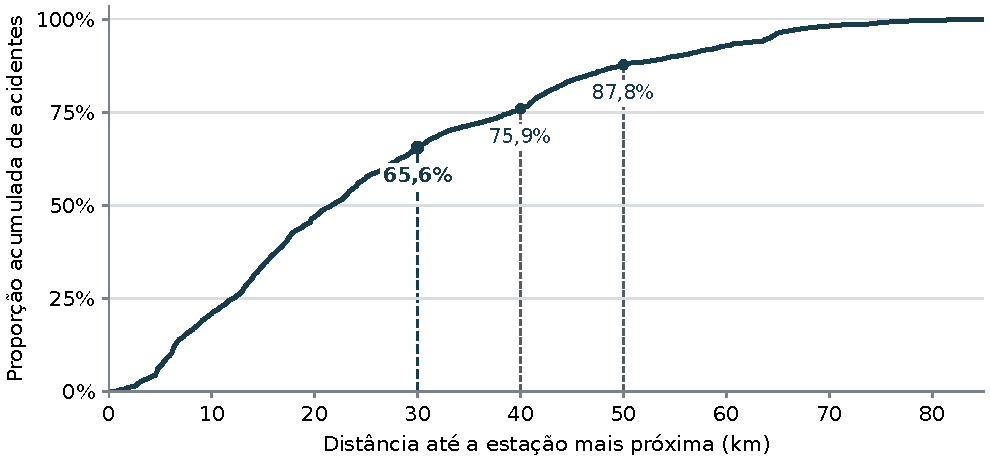
\includegraphics[width=0.87\linewidth]{cobertura_distancia.pdf}
    \caption{Cobertura acumulada por distância à estação mais próxima,
    antes do filtro de medição válida ($N=6.515$).}
    \label{fig:cobertura}
\end{figure}

Dos 6.515 acidentes, 854 (13,1\%) ficaram sem medição válida de
precipitação. A Tabela~\ref{tab:fluxo} mostra que o limite de 30 km
produziu a maior redução da amostra, com 1.931 exclusões entre os casos
com medição válida. O limite temporal de 60 minutos e o critério de
completude do desfecho e das covariáveis mantiveram a amostra em
3.730 acidentes (57,3\% da base integrada).

\begin{table}[H]
    \centering
    \caption{Seleção dos acidentes para a análise principal.}
    \label{tab:fluxo}
    \begin{tabular}{lrr}
        \toprule
        Etapa & Excluídos na etapa & Restantes \\
        \midrule
        Base integrada & \textemdash & 6.515 \\
        Com precipitação válida & 854 & 5.661 \\
        Distância até 30 km & 1.931 & 3.730 \\
        Diferença temporal até 60 min & 0 & 3.730 \\
        Desfecho e covariáveis completos & 0 & 3.730 \\
        \bottomrule
    \end{tabular}
\end{table}

As perdas variaram entre as estações. Em Registro,
por exemplo, houve 200 leituras ausentes entre 303 acidentes associados
à estação. A proporção sem leitura foi de 15,0\% no ano completo de 2025 e
de 8,4\% de janeiro a maio de 2026, recortes com coberturas sazonais
diferentes.

No diagnóstico ajustado da ausência, nenhum dos contrastes de gravidade
com os acidentes fatais como referência atingiu significância estatística.
A OR de ausência foi 0,726 para acidentes com vítimas feridas
(IC95\% 0,467-1,129, $p=0{,}155$) e 0,928 para acidentes sem vítimas
(IC95\% 0,567-1,517, $p=0{,}765$). O ajuste apresentou instabilidade em
algumas categorias sem variação na ausência. Os resultados são insuficientes
para estabelecer que a ausência ocorreu completamente ao acaso (MCAR) ou
ao acaso condicionalmente aos dados observados (MAR). Permanece a
possibilidade de viés de seleção na análise de casos completos.

Entre os 5.661 acidentes com medição válida, apenas 559 (9,9\%)
apresentaram precipitação acima de 0 mm, com máximo de 82,0 mm. A
concentração em zero e a presença de valores altos motivam a leitura
conjunta dos modelos para a presença de chuva e para a quantidade
registrada em milímetros.

A amostra principal reuniu 3.058 acidentes com vítimas feridas, 530
sem vítimas e 142 com vítimas fatais. Houve 402 acidentes com precipitação
superior a 0 mm (10,8\%) e 3.328 com precipitação igual a zero.
A Figura~\ref{fig:chuva_gravidade} apresenta a proporção de acidentes
com chuva por categoria de gravidade, sem ajuste por covariáveis. Os
nove acidentes fatais com chuva registrada pelo INMET limitam a precisão
das comparações para essa categoria.

\begin{figure}[H]
    \centering
    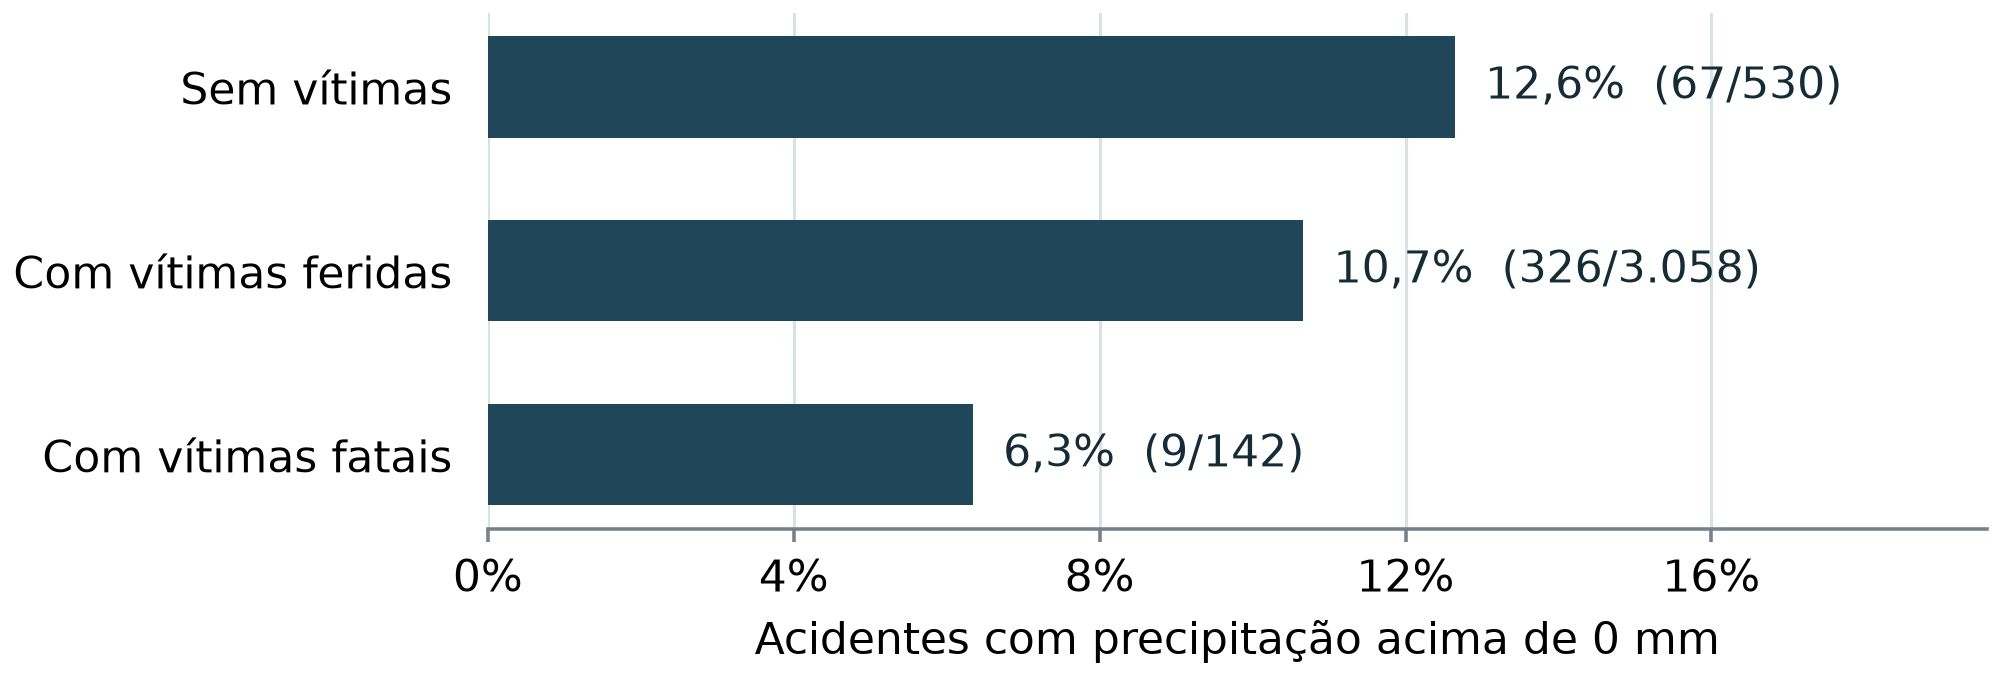
\includegraphics[width=0.87\linewidth]{chuva_gravidade.png}
    \caption{Proporção não ajustada de acidentes com precipitação acima de
    0 mm por gravidade na amostra principal ($N=3.730$).}
    \label{fig:chuva_gravidade}
\end{figure}

Os acidentes da amostra principal foram associados a 14 estações,
com 46,2\% dos registros vinculados à A701 e 71,2\% das ocorrências na
BR-116. Essa concentração limita a generalização para outros trechos.
Além disso, 398 acidentes compartilharam uma mesma leitura de estação
e horário com pelo menos outro acidente. O compartilhamento pode gerar
dependência entre observações, e os IC95\% dos modelos principais foram
calculados sem incorporação explícita desse agrupamento.

\subsection{Associação entre precipitação e gravidade}

A Tabela~\ref{tab:principal} apresenta as estimativas brutas e ajustadas
da regressão logística ordinal.

\begin{table}[H]
    \centering
    \caption{Regressões logísticas ordinais na amostra principal ($N=3.730$).}
    \label{tab:principal}
    \begin{tabular}{llrrr}
        \toprule
        Exposição & Modelo & OR & IC95\% & $p$ \\
        \midrule
        Precipitação (por mm) & Bruto    & 0,978 & 0,950-1,006 & 0,124 \\
        Chuva (sim vs.\ não)  & Bruto    & 0,766 & 0,592-0,991 & 0,042 \\
        Precipitação (por mm) & Ajustado & 0,977 & 0,949-1,006 & 0,123 \\
        Chuva (sim vs.\ não)  & Ajustado & 0,831 & 0,638-1,084 & 0,172 \\
        \bottomrule
    \end{tabular}
\end{table}

Para a precipitação contínua, a estimativa variou pouco após o ajuste.
A OR ajustada de 0,977 corresponde a chances cumulativas de maior
gravidade cerca de 2,3\% menores por milímetro adicional. O IC95\%
vai de chances cerca de 5\% menores a 0,6\% maiores.

Para chuva binária, a OR passou de 0,766 no modelo bruto para 0,831
no ajustado, cujo IC95\% incluiu 1. Na amostra principal, os modelos
ajustados não forneceram evidência estatisticamente significativa de
associação entre precipitação e gravidade em nenhuma das duas formas
de representar a exposição.

No diagnóstico exploratório de chances proporcionais, as ORs ajustadas
por milímetro foram 0,974 ($p=0{,}079$) para acidentes com vítimas
feridas ou fatais em relação aos sem vítimas e 1,009 ($p=0{,}786$)
para acidentes fatais em relação aos demais. No modelo ordinal
ajustado, a OR comum aos dois cortes foi de aproximadamente 0,977.
A diferença observada entre os cortes pode refletir, em parte, a
imprecisão das estimativas para acidentes fatais. Esse diagnóstico não
constitui um teste formal da hipótese de chances proporcionais.

Na regressão multinomial complementar, os acidentes sem vítimas
foram a categoria de referência. Para a precipitação contínua, as
ORs foram 0,973 para feridos (IC95\% 0,944-1,003, $p=0{,}075$) e
0,989 para fatais (IC95\% 0,924-1,058, $p=0{,}744$). Para chuva
binária, foram 0,899 (IC95\% 0,672-1,203, $p=0{,}474$) e 0,554
(IC95\% 0,265-1,159, $p=0{,}117$), respectivamente. Todos os
intervalos incluíram 1, assim como no modelo ordinal ajustado.
O intervalo mais amplo, no contraste de acidentes fatais para chuva
binária, admite associações de magnitudes bastante diferentes.

\subsection{Sensibilidades do pareamento}

As sensibilidades da Tabela~\ref{tab:robustez} avaliam três decisões
de pareamento. Ampliar o limite espacial muda a distância máxima aceita
e a composição da amostra. Alterar a regra temporal mantém os acidentes
e as estações, mas pode mudar a medição atribuída. Buscar uma estação
alternativa no mesmo horário acrescenta casos antes sem medição válida.

\begin{table}[H]
    \centering
    \caption{Sensibilidades do pareamento. Estimativas ordinais ajustadas.}
    \label{tab:robustez}
    \footnotesize
    \begin{tabular}{lrrr}
        \toprule
        Cenário & $N$ & \multicolumn{2}{c}{OR (IC95\%)} \\
        \cmidrule(lr){3-4}
                  &      & Precipitação (por mm) & Chuva (sim vs.\ não) \\
        \midrule
        \multicolumn{4}{l}{\textit{Limite espacial}} \\
        30 km (principal) & 3.730 & 0,977 (0,949-1,006) & 0,831 (0,638-1,084) \\
        40 km             & 4.339 & 0,978 (0,950-1,006) & 0,788 (0,616-1,008) \\
        50 km             & 5.015 & 0,976 (0,949-1,003) & 0,775 (0,615-0,978) \\
        \addlinespace
        \multicolumn{4}{l}{\textit{Horários nos mesmos acidentes}} \\
        A: horário mais próximo  & 3.700 & 0,977 (0,949-1,006) & 0,839 (0,642-1,095) \\
        B: intervalo do acidente & 3.700 & 0,961 (0,919-1,004) & 0,785 (0,599-1,028) \\
        C: última hora encerrada & 3.700 & 0,981 (0,952-1,012) & 0,805 (0,618-1,049) \\
        \addlinespace
        Estação alternativa, horário A & 3.891 & 0,976 (0,948-1,005) & 0,773 (0,597-1,001) \\
        \bottomrule
    \end{tabular}
\end{table}

Ao ampliar o limite de 30 para 40 e 50 km, as estimativas por
milímetro permaneceram semelhantes, com IC95\% incluindo 1 nos três
cenários. Para chuva binária, as ORs ajustadas se afastaram de 1.
O IC95\% ainda incluiu 1 a 40 km ($p=0{,}058$) e ficou abaixo de 1
a 50 km ($p=0{,}032$). O cenário de 50 km admite medições mais distantes
e acrescenta 1.285 acidentes, de modo que a variação da estimativa
também pode refletir a composição da amostra. O limite de 30 km
permaneceu como referência, e o resultado a 50 km foi interpretado
como parte da análise de sensibilidade.

Entre os 3.700 acidentes com leitura válida nas três regras temporais,
398 tiveram chuva pela regra A, 381 pela regra B e 406 pela regra C.
Em relação a A, B reclassificou 169 acidentes (4,57\%), com 76
mudanças para chuva e 93 para ausência de chuva. C reclassificou 124
(3,35\%), com 66 mudanças para chuva e 58 para ausência de chuva.
Assim, a classificação de um mesmo acidente pode variar com o intervalo
de acumulação escolhido. Os IC95\% para ambas as exposições incluíram
1 nas três regras.

A busca por uma estação alternativa com leitura válida no horário
original recuperou 161 acidentes, dos quais nove tiveram chuva.
A amostra passou de 3.730 para 3.891 acidentes, e o total com chuva
subiu de 402 para 411. Entre os casos recuperados, a distância mediana
passou de 16,4 para 19,1 km, com aumento mediano individual de 2,7 km.
Os acidentes previamente medidos conservaram tanto o valor em
milímetros quanto a classificação de chuva. A mudança das estimativas
decorreu, portanto, da inclusão dos casos recuperados.

Nesse cenário, a OR por milímetro permaneceu próxima à principal
($p=0{,}100$). Para chuva binária, a OR passou de 0,831 para 0,773
($p=0{,}051$), com IC95\% ainda incluindo 1. No conjunto das
sensibilidades, as estimativas por milímetro variaram relativamente
pouco e seus intervalos incluíram 1. As estimativas binárias
variaram mais com as regras de pareamento e a composição da amostra.

\Needspace{7\baselineskip}
\subsection{Comparação complementar PRF-INMET}

Até 30 km da estação mais próxima, havia 3.679 acidentes com
classificação válida de chuva nas duas fontes. A Tabela~\ref{tab:prf-inmet}
mostra que as classificações coincidiram em 89,0\% dos casos. Esse
percentual reflete, em grande parte, o predomínio de registros sem
chuva nas duas fontes. A concordância específica foi de 93,7\% para
ausência de chuva e de 58,9\% para presença de chuva.

\begin{table}[H]
    \centering
    \caption{Classificações de chuva pela PRF e pelo INMET até 30 km.}
    \label{tab:prf-inmet}
    \begin{tabular}{lrrr}
        \toprule
        PRF & INMET sem chuva & INMET com chuva & Total \\
        \midrule
        Sem registro explícito de chuva & 2.986 & 107 & 3.093 \\
        Chuva ou garoa & 297 & 289 & 586 \\
        \midrule
        Total & 3.283 & 396 & 3.679 \\
        \bottomrule
    \end{tabular}
\end{table}

Os dois indicadores tenderam a variar na mesma direção, com correlação
positiva e moderada ($r=\phi=0{,}541$, IC95\% exploratório por estação
de 0,473 a 0,571, $p$ nominal $<0{,}001$). Já o $\kappa$ de Cohen de
0,528 indicou concordância moderada além da esperada ao acaso.
O valor nominal de $p$ para a associação deve ser interpretado com
cautela diante da possível dependência entre acidentes associados
à mesma estação. A PRF registra a condição meteorológica no contexto
da ocorrência, enquanto o INMET mede a precipitação acumulada na
estação. A comparação considera as duas fontes sem adotar um
padrão-ouro.

\begin{table}[H]
    \centering
    \caption{Associação e concordância PRF-INMET por limite espacial.}
    \label{tab:concordancia}
    \footnotesize
    \begin{tabular}{rrrrrrr}
        \toprule
        & & & & \multicolumn{3}{c}{Concordância} \\
        \cmidrule(lr){5-7}
        Limite & $N$ & $\phi$ (IC95\%) & $\kappa$ & Total & Chuva (específica) & Ausência (específica) \\
        \midrule
        10 km & 1.227 & 0,597 (0,477-0,651) & 0,591 & 92,7\% & 63,1\% & 95,9\% \\
        20 km & 2.612 & 0,556 (0,464-0,611) & 0,544 & 90,0\% & 59,9\% & 94,3\% \\
        30 km & 3.679 & 0,541 (0,473-0,571) & 0,528 & 89,0\% & 58,9\% & 93,7\% \\
        \bottomrule
    \end{tabular}
    \par\smallskip
    {\footnotesize $p$ nominal de Pearson/$\phi$ $<0{,}001$ nos três recortes.
    IC95\% exploratório por estação.}
\end{table}

Os valores de $\phi$ e $\kappa$ foram maiores nos recortes mais
próximos (Tabela~\ref{tab:concordancia}). Os recortes incluem
conjuntos diferentes de acidentes, e os IC95\% exploratórios de
$\phi$ se sobrepõem. A comparação descreve o padrão observado,
sem isolar a contribuição da distância.

Nos mesmos 3.679 acidentes, as ORs binárias ajustadas foram 0,826
para o INMET (IC95\% 0,633-1,080, $p=0{,}162$) e 0,906 para a
PRF (IC95\% 0,712-1,153, $p=0{,}423$). Como ambos os intervalos
incluíram 1, a interpretação inferencial se manteve nessa amostra
com as duas fontes.

As estimativas devem ser interpretadas à luz da cobertura e da
resolução das medições e das variáveis disponíveis para o ajuste,
que não incluem o volume de tráfego ou a velocidade no momento da
ocorrência. O estudo avalia a gravidade entre os acidentes
registrados pela PRF e não estima o risco de ocorrência de acidentes
em situações com ou sem chuva.

\section{Conclusão}

Este trabalho avaliou a associação entre precipitação horária e gravidade
entre os acidentes registrados em rodovias federais do estado de São Paulo,
a partir da integração de dados da PRF com medições de estações automáticas
do INMET. Na análise principal de 3.730 acidentes, os modelos logísticos
ordinais ajustados não forneceram evidência estatisticamente significativa
de associação com a gravidade, tanto para a precipitação contínua quanto
para o indicador binário de chuva. Os intervalos de confiança incluíram 1
e admitem associações de diferentes magnitudes.

A regressão multinomial complementar levou a uma interpretação semelhante.
Nas sensibilidades, as estimativas por milímetro permaneceram relativamente estáveis.
A comparação entre PRF e INMET mostrou concordância moderada além do acaso,
com maior concordância específica para a ausência de chuva, e os modelos
ajustados com os indicadores das duas fontes levaram à mesma interpretação
inferencial na amostra comparável.

As perdas de medições, a resolução horária, a distância às estações e a
concentração das ocorrências em determinadas estações e rodovias limitam
a interpretação dos resultados. O estudo analisa a gravidade entre os
acidentes registrados pela PRF e não estima o risco de ocorrência de
acidentes em situações com ou sem chuva. A comparação entre as regras de
pareamento mostrou que a classificação de chuva para um mesmo acidente pode
variar com o intervalo horário adotado. As estimativas para o indicador
binário também variaram mais do que as estimativas por milímetro quando os
critérios espaciais e a recuperação de medições alteraram a composição da
amostra.

\begingroup
\raggedright
\bibliographystyle{sbc}
\bibliography{sbc-template}
\endgroup

\end{document}
